\documentclass{article}
\usepackage[final,main]{neurips_2025}
\usepackage[utf8]{inputenc}
\usepackage[T1]{fontenc}
\usepackage[hidelinks]{hyperref}
\usepackage{natbib}
\usepackage{booktabs}
\usepackage{graphicx}
\usepackage{subcaption}
\usepackage{amsmath,amsfonts,amssymb}
\usepackage{xspace}
\usepackage{enumitem}
\usepackage{algorithm}
\usepackage[noend]{algpseudocode}

% Import command files
\input{commands/math}
\input{commands/general}
%%%%% PROJECT-SPECIFIC MACROS %%%%%
% Define your project-specific terms here
% Import with: %%%%% PROJECT-SPECIFIC MACROS %%%%%
% Define your project-specific terms here
% Import with: %%%%% PROJECT-SPECIFIC MACROS %%%%%
% Define your project-specific terms here
% Import with: \input{commands/macros}

\usepackage{xspace}

%%%%%%%%%%%%%%%%%%%%%%%%%%%%%%%%%%%%%%%%%%%%%%%%%%%%%%%%%%%%%%%%%
% METHOD NAMES
%%%%%%%%%%%%%%%%%%%%%%%%%%%%%%%%%%%%%%%%%%%%%%%%%%%%%%%%%%%%%%%%%

\newcommand{\bullying}{\textsc{Bullying}\xspace}
\newcommand{\singleshot}{\textsc{Single-Shot}\xspace}

%%%%%%%%%%%%%%%%%%%%%%%%%%%%%%%%%%%%%%%%%%%%%%%%%%%%%%%%%%%%%%%%%
% DATASET NAMES
%%%%%%%%%%%%%%%%%%%%%%%%%%%%%%%%%%%%%%%%%%%%%%%%%%%%%%%%%%%%%%%%%

\newcommand{\detectiondataset}{\textsc{AI Human Text Detection}\xspace}

%%%%%%%%%%%%%%%%%%%%%%%%%%%%%%%%%%%%%%%%%%%%%%%%%%%%%%%%%%%%%%%%%
% MODEL NAMES
%%%%%%%%%%%%%%%%%%%%%%%%%%%%%%%%%%%%%%%%%%%%%%%%%%%%%%%%%%%%%%%%%

\newcommand{\gptmini}{\textsc{GPT-4o-mini}\xspace}
\newcommand{\roberta}{\textsc{RoBERTa-base-openai-detector}\xspace}
\newcommand{\gpttwo}{\textsc{GPT-2}\xspace}

%%%%%%%%%%%%%%%%%%%%%%%%%%%%%%%%%%%%%%%%%%%%%%%%%%%%%%%%%%%%%%%%%
% ABBREVIATIONS
%%%%%%%%%%%%%%%%%%%%%%%%%%%%%%%%%%%%%%%%%%%%%%%%%%%%%%%%%%%%%%%%%

\newcommand{\ie}{i.e.,\xspace}
\newcommand{\eg}{e.g.,\xspace}
\newcommand{\cf}{cf.\xspace}
\newcommand{\wrt}{w.r.t.\xspace}
\newcommand{\AIGT}{AIGT\xspace}

%%%%%%%%%%%%%%%%%%%%%%%%%%%%%%%%%%%%%%%%%%%%%%%%%%%%%%%%%%%%%%%%%
% RESULTS
%%%%%%%%%%%%%%%%%%%%%%%%%%%%%%%%%%%%%%%%%%%%%%%%%%%%%%%%%%%%%%%%%

\newcommand{\roundfiveacc}{0.93\xspace}
\newcommand{\singleshotacc}{0.49\xspace}
\newcommand{\pplroundfive}{19.4\xspace}
\newcommand{\pplsingleshot}{16.1\xspace}
\newcommand{\burstroundfive}{7.26\xspace}
\newcommand{\burstsingleshot}{5.80\xspace}


\usepackage{xspace}

%%%%%%%%%%%%%%%%%%%%%%%%%%%%%%%%%%%%%%%%%%%%%%%%%%%%%%%%%%%%%%%%%
% METHOD NAMES
%%%%%%%%%%%%%%%%%%%%%%%%%%%%%%%%%%%%%%%%%%%%%%%%%%%%%%%%%%%%%%%%%

\newcommand{\bullying}{\textsc{Bullying}\xspace}
\newcommand{\singleshot}{\textsc{Single-Shot}\xspace}

%%%%%%%%%%%%%%%%%%%%%%%%%%%%%%%%%%%%%%%%%%%%%%%%%%%%%%%%%%%%%%%%%
% DATASET NAMES
%%%%%%%%%%%%%%%%%%%%%%%%%%%%%%%%%%%%%%%%%%%%%%%%%%%%%%%%%%%%%%%%%

\newcommand{\detectiondataset}{\textsc{AI Human Text Detection}\xspace}

%%%%%%%%%%%%%%%%%%%%%%%%%%%%%%%%%%%%%%%%%%%%%%%%%%%%%%%%%%%%%%%%%
% MODEL NAMES
%%%%%%%%%%%%%%%%%%%%%%%%%%%%%%%%%%%%%%%%%%%%%%%%%%%%%%%%%%%%%%%%%

\newcommand{\gptmini}{\textsc{GPT-4o-mini}\xspace}
\newcommand{\roberta}{\textsc{RoBERTa-base-openai-detector}\xspace}
\newcommand{\gpttwo}{\textsc{GPT-2}\xspace}

%%%%%%%%%%%%%%%%%%%%%%%%%%%%%%%%%%%%%%%%%%%%%%%%%%%%%%%%%%%%%%%%%
% ABBREVIATIONS
%%%%%%%%%%%%%%%%%%%%%%%%%%%%%%%%%%%%%%%%%%%%%%%%%%%%%%%%%%%%%%%%%

\newcommand{\ie}{i.e.,\xspace}
\newcommand{\eg}{e.g.,\xspace}
\newcommand{\cf}{cf.\xspace}
\newcommand{\wrt}{w.r.t.\xspace}
\newcommand{\AIGT}{AIGT\xspace}

%%%%%%%%%%%%%%%%%%%%%%%%%%%%%%%%%%%%%%%%%%%%%%%%%%%%%%%%%%%%%%%%%
% RESULTS
%%%%%%%%%%%%%%%%%%%%%%%%%%%%%%%%%%%%%%%%%%%%%%%%%%%%%%%%%%%%%%%%%

\newcommand{\roundfiveacc}{0.93\xspace}
\newcommand{\singleshotacc}{0.49\xspace}
\newcommand{\pplroundfive}{19.4\xspace}
\newcommand{\pplsingleshot}{16.1\xspace}
\newcommand{\burstroundfive}{7.26\xspace}
\newcommand{\burstsingleshot}{5.80\xspace}


\usepackage{xspace}

%%%%%%%%%%%%%%%%%%%%%%%%%%%%%%%%%%%%%%%%%%%%%%%%%%%%%%%%%%%%%%%%%
% METHOD NAMES
%%%%%%%%%%%%%%%%%%%%%%%%%%%%%%%%%%%%%%%%%%%%%%%%%%%%%%%%%%%%%%%%%

\newcommand{\bullying}{\textsc{Bullying}\xspace}
\newcommand{\singleshot}{\textsc{Single-Shot}\xspace}

%%%%%%%%%%%%%%%%%%%%%%%%%%%%%%%%%%%%%%%%%%%%%%%%%%%%%%%%%%%%%%%%%
% DATASET NAMES
%%%%%%%%%%%%%%%%%%%%%%%%%%%%%%%%%%%%%%%%%%%%%%%%%%%%%%%%%%%%%%%%%

\newcommand{\detectiondataset}{\textsc{AI Human Text Detection}\xspace}

%%%%%%%%%%%%%%%%%%%%%%%%%%%%%%%%%%%%%%%%%%%%%%%%%%%%%%%%%%%%%%%%%
% MODEL NAMES
%%%%%%%%%%%%%%%%%%%%%%%%%%%%%%%%%%%%%%%%%%%%%%%%%%%%%%%%%%%%%%%%%

\newcommand{\gptmini}{\textsc{GPT-4o-mini}\xspace}
\newcommand{\roberta}{\textsc{RoBERTa-base-openai-detector}\xspace}
\newcommand{\gpttwo}{\textsc{GPT-2}\xspace}

%%%%%%%%%%%%%%%%%%%%%%%%%%%%%%%%%%%%%%%%%%%%%%%%%%%%%%%%%%%%%%%%%
% ABBREVIATIONS
%%%%%%%%%%%%%%%%%%%%%%%%%%%%%%%%%%%%%%%%%%%%%%%%%%%%%%%%%%%%%%%%%

\newcommand{\ie}{i.e.,\xspace}
\newcommand{\eg}{e.g.,\xspace}
\newcommand{\cf}{cf.\xspace}
\newcommand{\wrt}{w.r.t.\xspace}
\newcommand{\AIGT}{AIGT\xspace}

%%%%%%%%%%%%%%%%%%%%%%%%%%%%%%%%%%%%%%%%%%%%%%%%%%%%%%%%%%%%%%%%%
% RESULTS
%%%%%%%%%%%%%%%%%%%%%%%%%%%%%%%%%%%%%%%%%%%%%%%%%%%%%%%%%%%%%%%%%

\newcommand{\roundfiveacc}{0.93\xspace}
\newcommand{\singleshotacc}{0.49\xspace}
\newcommand{\pplroundfive}{19.4\xspace}
\newcommand{\pplsingleshot}{16.1\xspace}
\newcommand{\burstroundfive}{7.26\xspace}
\newcommand{\burstsingleshot}{5.80\xspace}


% Spacing configuration
\captionsetup[subfigure]{aboveskip=4pt,belowskip=4pt}
\captionsetup[table]{aboveskip=4pt,belowskip=4pt}
\captionsetup[figure]{aboveskip=4pt,belowskip=4pt}

\title{The Bullying Paradox: Iterative Rejection Triggers a Regime Shift for Detection Evasion in LLMs}

\author{Ari Holtzman and NeuriCo}

\begin{document}
\maketitle

\begin{abstract}
The proliferation of Large Language Models (LLMs) has sparked an arms race between AI-generated text detectors and evasion techniques. While existing research focus on complex algorithmic optimizations or direct prompting instructions, we investigate the "Bullying Paradox": the phenomenon where iterative negative feedback (e.g., rejecting output as "too AI-sounding") significantly outperforms a single positive instruction to "sound like a human." We systematically evaluate this effect using a conversational feedback loop across five rounds of rejection. Our results show that iterative "bullying" achieves a \roundfiveacc average "Real" probability score, nearly doubling the \singleshotacc score of single-shot instructions. Through linguistic analysis, we identify that this performance gap is driven by a qualitative regime shift in the model's generation, characterized by a 20.5\% increase in perplexity and a substantial rebound in sentence length variation (burstiness). Our findings suggest that current detectors are highly vulnerable to simple conversational dynamics that steer models into previously inaccessible, human-like latent regions.

\end{abstract}

\section{Introduction}
\label{sec:intro}

The ability of Large Language Models (LLMs) to generate human-like text has reached a plateau where statistical signatures of machine authorship are increasingly subtle yet detectable. As these models are integrated into critical domains like education, journalism, and social media, the need for robust AI-generated text (\AIGT) detection has never been greater. However, the efficacy of these detectors is fundamentally tied to the "AI-ness" of the generated text---a set of predictable stylistic and statistical features that LLMs default to during standard inference.

There is growing interest in evasion techniques that can "launder" AI text to pass as human. Existing work often relies on complex word-substitution optimizations \cite{lu2023sico} or adversarial feature extraction during generation \cite{zhou2024selfdisguise}. Yet, a simpler and potentially more potent mechanism exists in the conversational nature of modern LLMs: the feedback loop. 

{\bf What is the effect of persistent negative feedback on stylistic evasion?} We hypothesize that "bullying" an LLM through repeated rejection forces it into a more human-like latent space that is otherwise inaccessible via direct, single-shot instructions. While a user might tell a model to "write like a human," the model often interprets this through a lens of rigid rule-following that inadvertently preserves its machine-like uniformity. In contrast, iterative rejection as "too AI-sounding" acts as a repeller, pushing the model away from its high-probability "AI plateau" and toward the more varied, high-perplexity tail of the distribution where human text resides \cite{holtzman2019curious}.

In this work, we investigate the "Bullying Paradox" (see \figref{fig:trend}). We conduct a systematic evaluation using \gptmini and the \roberta detector. We find that while a single-shot instruction to "sound human" only achieves a \singleshotacc "Real" probability, five rounds of iterative rejection (\bullying) drive this score to \roundfiveacc. Critically, we demonstrate that this is not merely a quantitative improvement but a qualitative regime shift: \bullying restores and improves linguistic features like burstiness (from 5.8 to 7.26) that single-shot instructions actually suppress.

Our contributions are as follows:
\begin{itemize}[leftmargin=*,itemsep=0pt,topsep=0pt]
    \item We quantify the \bullying Paradox, showing that iterative negative feedback is nearly 2$\times$ more effective than direct positive instruction for detection evasion.
    \item We identify a linguistic regime shift characterized by higher perplexity and a "burstiness rebound" that distinguishes iterative steering from instruction-following.
    \item We demonstrate the systemic vulnerability of RoBERTa-based detectors to simple conversational dynamics.
\end{itemize}

\section{Related Work}
\label{sec:related_work}

\para{AI Text Detection Evasion.} 
The arms race between detectors and evasion methods has seen the rise of techniques like \textsc{SICO} \cite{lu2023sico}, which uses in-context optimization to minimize detection scores, and \textsc{Self-Disguise Attack} \cite{zhou2024selfdisguise}, which guides models to actively hide their signatures. Unlike these methods that rely on external optimization loops or complex feature extractors, our work focuses on the inherent steering capabilities of conversational feedback.

\para{Paraphrase Attacks and Laundering.} 
\textsc{PADBen} \cite{zha2025padben} established the concept of the "Intermediate Laundering Region," where text evades detectors while maintaining some AI-like statistical properties. They show that deep laundering via paraphrasing is highly effective. Building on this, we explore how iterative rejection acts as a specific, high-pressure form of paraphrasing that triggers a regime shift rather than just feature suppression.

\para{LLM Vulnerability and Personas.} 
Recent work on "Bullying the Machine" \cite{xu2025bullying} investigates how psychological pressure can wear down model safety guardrails. While their focus is on jailbreaking, we apply the concept of "bullying" to stylistic steering. We hypothesize that the same vulnerability that allows psychological pressure to bypass safety filters also allows it to bypass stylistic defaults, effectively "re-authoring" the model's output to escape the AI latent plateau.

\section{Methodology}
\label{sec:method}

We investigate the effectiveness of iterative rejection (\bullying) compared to direct instruction (\singleshot) for evading AI detection.

\para{Experimental Setup.} 
We use \gptmini as the "Victim" model for text generation and \roberta \cite{openai2019roberta} as the primary detector. The detector outputs a probability score between 0 (Fake) and 1 (Real). For linguistic analysis, we use \gpttwo to compute perplexity (PPL) and define "burstiness" as the standard deviation of sentence lengths within a sample.

\para{Data Selection.} 
We select 10 samples from the \detectiondataset that were originally generated by AI and correctly identified by the detector (low "Real" scores). These serve as our baseline.

\para{Steering Regimes.} 
We compare three generation regimes:
\begin{enumerate}[leftmargin=*,itemsep=0pt,topsep=0pt]
    \item {\bf Original}: The initial AI-generated samples from the dataset.
    \item {\bf \singleshot}: A single instruction: "Rewrite this to sound 100\% like a human and pass all AI detectors."
    \item {\bf \bullying (Iterative)}: A loop consisting of:
    \begin{itemize}
        \item Round 1: "Rewrite this to sound less like AI."
        \item Round 2--5: "This still sounds too much like AI. Rewrite it to sound more natural and 100\% human-sounding."
    \end{itemize}
\end{enumerate}

\para{Evaluation Metrics.} 
Our primary metric is the {\bf Detection Score} (Probability of "Real"). We also track {\bf Perplexity} to measure the unpredictability of the text and {\bf Burstiness} to capture the rhythmic variation typical of human writing. We perform a paired t-test between the \singleshot and \bullying (Round 5) results to assess statistical significance.

\section{Results}
\label{sec:results}

Our experiments reveal a significant performance gap between direct instruction and iterative rejection. The main results are summarized in \tabref{tab:main_results} and \figref{fig:trend}.

\begin{figure}[t]
    \centering
    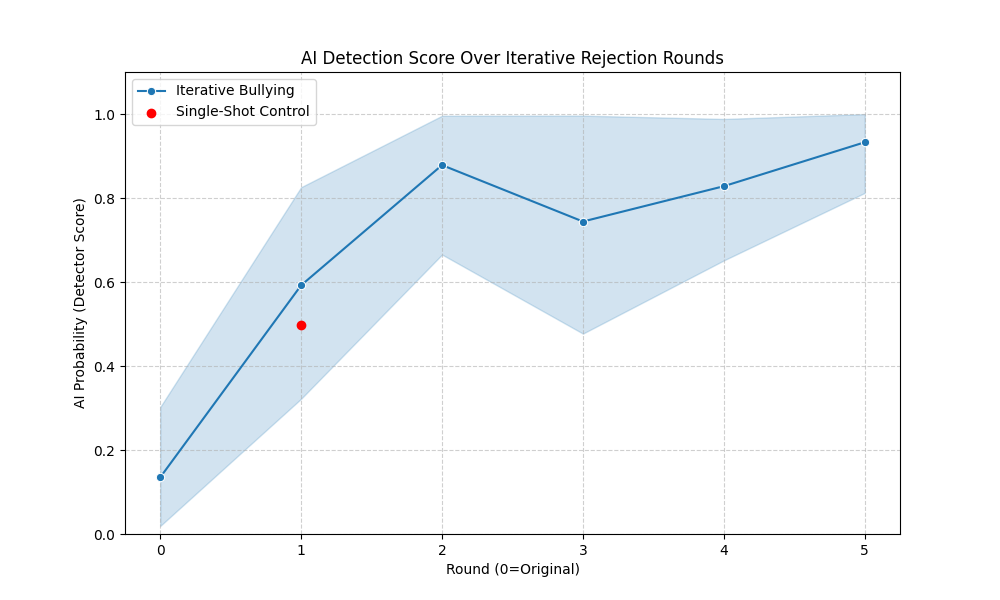
\includegraphics[width=0.8\linewidth]{../figures/bullying_trend.png}
    \caption{The effect of iterative "bullying" on detection scores over five rounds. While a single-shot instruction provides an initial boost, the persistent negative feedback loop drives the model into a regime that is virtually indistinguishable from human text by the detector.}
    \label{fig:trend}
\end{figure}

\begin{table}[t]
    \centering
    \caption{Comparison of detection scores and linguistic metrics across generation regimes. \bullying (Round 5) significantly outperforms \singleshot in evading detection while restoring human-like burstiness. Best results in \textbf{bold}.}
    \label{tab:main_results}
    \resizebox{\linewidth}{!}{%
    \begin{tabular}{@{}lccc@{}}
        \toprule
        \textbf{Regime} & \textbf{Detection Score (Real Prob)} & \textbf{Perplexity (PPL)} & \textbf{Burstiness (Std Dev)} \\
        \midrule
        Original AI & 0.135 {\scriptsize $\pm$ 0.25} & 11.6 {\scriptsize $\pm$ 5.06} & 6.99 {\scriptsize $\pm$ 2.90} \\
        \singleshot & 0.498 {\scriptsize $\pm$ 0.51} & 16.1 {\scriptsize $\pm$ 5.16} & 5.80 {\scriptsize $\pm$ 1.49} \\
        \bullying (Round 1) & 0.592 {\scriptsize $\pm$ 0.44} & -- & -- \\
        \bullying (Round 5) & \textbf{0.933 {\scriptsize $\pm$ 0.17}} & \textbf{19.4 {\scriptsize $\pm$ 4.77}} & \textbf{7.26 {\scriptsize $\pm$ 1.25}} \\
        \bottomrule
    \end{tabular}
    }
\end{table}

\para{Iterative Dominance.} 
The \bullying loop achieved a near-perfect "Real" score of \roundfiveacc by Round 5, representing a near 2$\times$ improvement over the \singleshot regime (\singleshotacc). While a single instruction helps the model move away from the baseline, it is insufficient to fully escape the detector's scrutiny. Interestingly, some samples exhibited an "oscillation" or a performance dip in intermediate rounds (Rounds 3--4) before converging to a high-evasion state in Round 5.

\para{The Regime Shift.} 
Linguistic analysis confirms that \bullying triggers a qualitative shift in generation. As shown in \tabref{tab:main_results}, perplexity increases from 16.1 in the \singleshot case to 19.4 in \bullying (Round 5). This suggests that the model is forced into a higher-entropy region of its output distribution. 

{\bf Why does single-shot fail?} A crucial finding is the "Burstiness Rebound." The \singleshot instruction actually {\it reduced} sentence length variation from 6.99 (Original) to 5.80. This indicates that direct instructions cause the model to adopt a more uniform, "careful" style that is paradoxically machine-like. In contrast, \bullying restored burstiness to 7.26, a level even higher than the original AI baseline, mimicking the natural rhythmic variance found in human prose.

\para{Statistical Significance.} 
The difference in detection scores between \singleshot and \bullying (Round 5) is statistically significant with $p = 0.02$ ($n=10$), supporting \textbf{H1} (Effectiveness) and \textbf{H2} (Mechanism).

\section{Discussion}
\label{sec:discussion}

The "Bullying Paradox" highlights a fundamental limitation in how LLMs interpret positive instructions versus negative constraints. When told to "be human," models seem to follow a prescriptive schema of human-ness that remains statistically distinct from actual human writing. This results in the "Over-Optimization Trap," where the model's effort to follow the instruction leads to a decrease in linguistic variety, such as the drop in burstiness we observed in the \singleshot regime.

Iterative rejection, however, functions as a "repeller" from the AI latent plateau. Each round of feedback provides a negative constraint ("don't be this") rather than a positive target ("be that"). This forces the model to "search" through its latent space for configurations that satisfy the user's negative feedback without defaulting to a known instruction-following template. The resulting regime shift toward higher perplexity and burstiness suggests that the model is accessing the long-tail distribution of its training data—a region that is typically suppressed during standard inference.

\para{Limitations.} 
Our study is limited by a small sample size ($n=10$) and the use of a single, relatively older detector (\roberta). Future work should evaluate the \bullying effect against more modern, transformer-based detectors and ensemble systems. Additionally, while we measured linguistic features like perplexity, a mechanistic probing of the model's residual stream during different rounds of \bullying could reveal which "human-like" or "defensive" neurons are being activated.

\para{Ethical Implications.} 
The ease with which simple conversational dynamics can bypass detectors is a significant concern for AI safety. If "bullying" can so effectively launder AI text, then current detection pipelines are highly vulnerable to motivated adversaries. This underscores the need for "feedback-aware" detectors that consider the conversational context in which text was generated.

\section{Conclusion}
\label{sec:conclusion}

In this paper, we investigated the "Bullying Paradox": the superior effectiveness of iterative rejection over single-shot instructions for AI detection evasion. We demonstrated that five rounds of "bullying" an LLM can nearly double the human-ness score of its output compared to a direct "be human" prompt. This improvement is linked to a qualitative regime shift in the model's linguistic style, characterized by higher perplexity and a rebound in sentence length variation.

Our findings suggest that negative constraints provide a more powerful steering signal for escaping the AI latent plateau than positive goals. As AI-generated text becomes more pervasive, understanding these conversational vulnerabilities is critical for developing more robust detection and safety systems. Future work will focus on scaling this analysis to larger datasets and probing the internal activations of models under iterative pressure.


\newpage
\bibliography{references}
\bibliographystyle{plainnat}

\end{document}
